\documentclass[a4paper,12pt]{article}
%\usepackage{fullpage}
%\usepackage{pdfpages}

\usepackage{geometry}
 \geometry{
 a4paper,
 total={170mm,257mm},
 left=20mm,
 top=20mm,
 }

\usepackage{color}
\usepackage{amsmath,graphicx,makeidx}
\usepackage{lscape}
\usepackage{fancyhdr}
\addtolength{\headheight}{1.5cm} % make more space for the header
\pagestyle{fancyplain} % use fancy for all pages except chapter start
\lhead{
\includegraphics[height=1.7cm]{FOSSEE-logo}} % left logo
\rhead{
\includegraphics[height=3.5cm]{DWSIM-flowsheeting-project-logo}} % right logo
\renewcommand{\headrulewidth}{0pt} % remove rule below header

\title{Production of Biodiesel}
\author{Daniel Wagner \\ DWSIM Developer}
\date{}

\begin{document}

\maketitle

\noindent \textbf{Background \& Description:}
\newline Biodiesel was introduced in South Africa before World War II to power heavy-duty vehicles. Recent environmental and domestic economic concerns have prompted a resurgence in the use of biodiesel throughout the world. Biodiesel can be produced through "transesterification"; a process that combines vegetable oils, animal fats, and/or microalgae oils with alcohol in the presence of a catalyst to form fatty esters. Products are separated into phases which provide easy removal of glycerol, a valuable industrial by-product, in the first phase. The remaining alcohol/ester mixture is then separated and the excess alcohol is recycled. Then the esters are sent to the clean-up or purification processes, which consist of water washing, vacuum drying, and filtration. 

In this flowsheet, production of ethyl palmitate ($C_{18}H_{36}O_2$) from tripalmitin ($C_{51}H_{98}O_6$) has been demonstrated. Ethyl palmitate is a colourless solid with a wax-like odour. Chemically, ethyl palmitate is the ethyl ester of palmitic acid. Ethyl palmitate is used as a hair- and skin-conditioning agent. Tripalmitin feed along with ethanol is sent to a conversion reactor where reaction takes place between tripalmitin and ethanol to form ethyl palmitate and glycerol. The reactor is considered to have 95\% conversion of tripalmitin. The product stream is first sent to a distillation column for ethanol separation. Ethanol recovered from top is recycled back to the mix with the feed stream. The bottom stream containing biodiesel along with other impurities are sent to an absorption column. Water is sent to the bottom of the column to absorb the other impurities from biodiesel while pure Ethyl Palmitate is obtained from the bottom.

\vspace{7ex}
\centerline{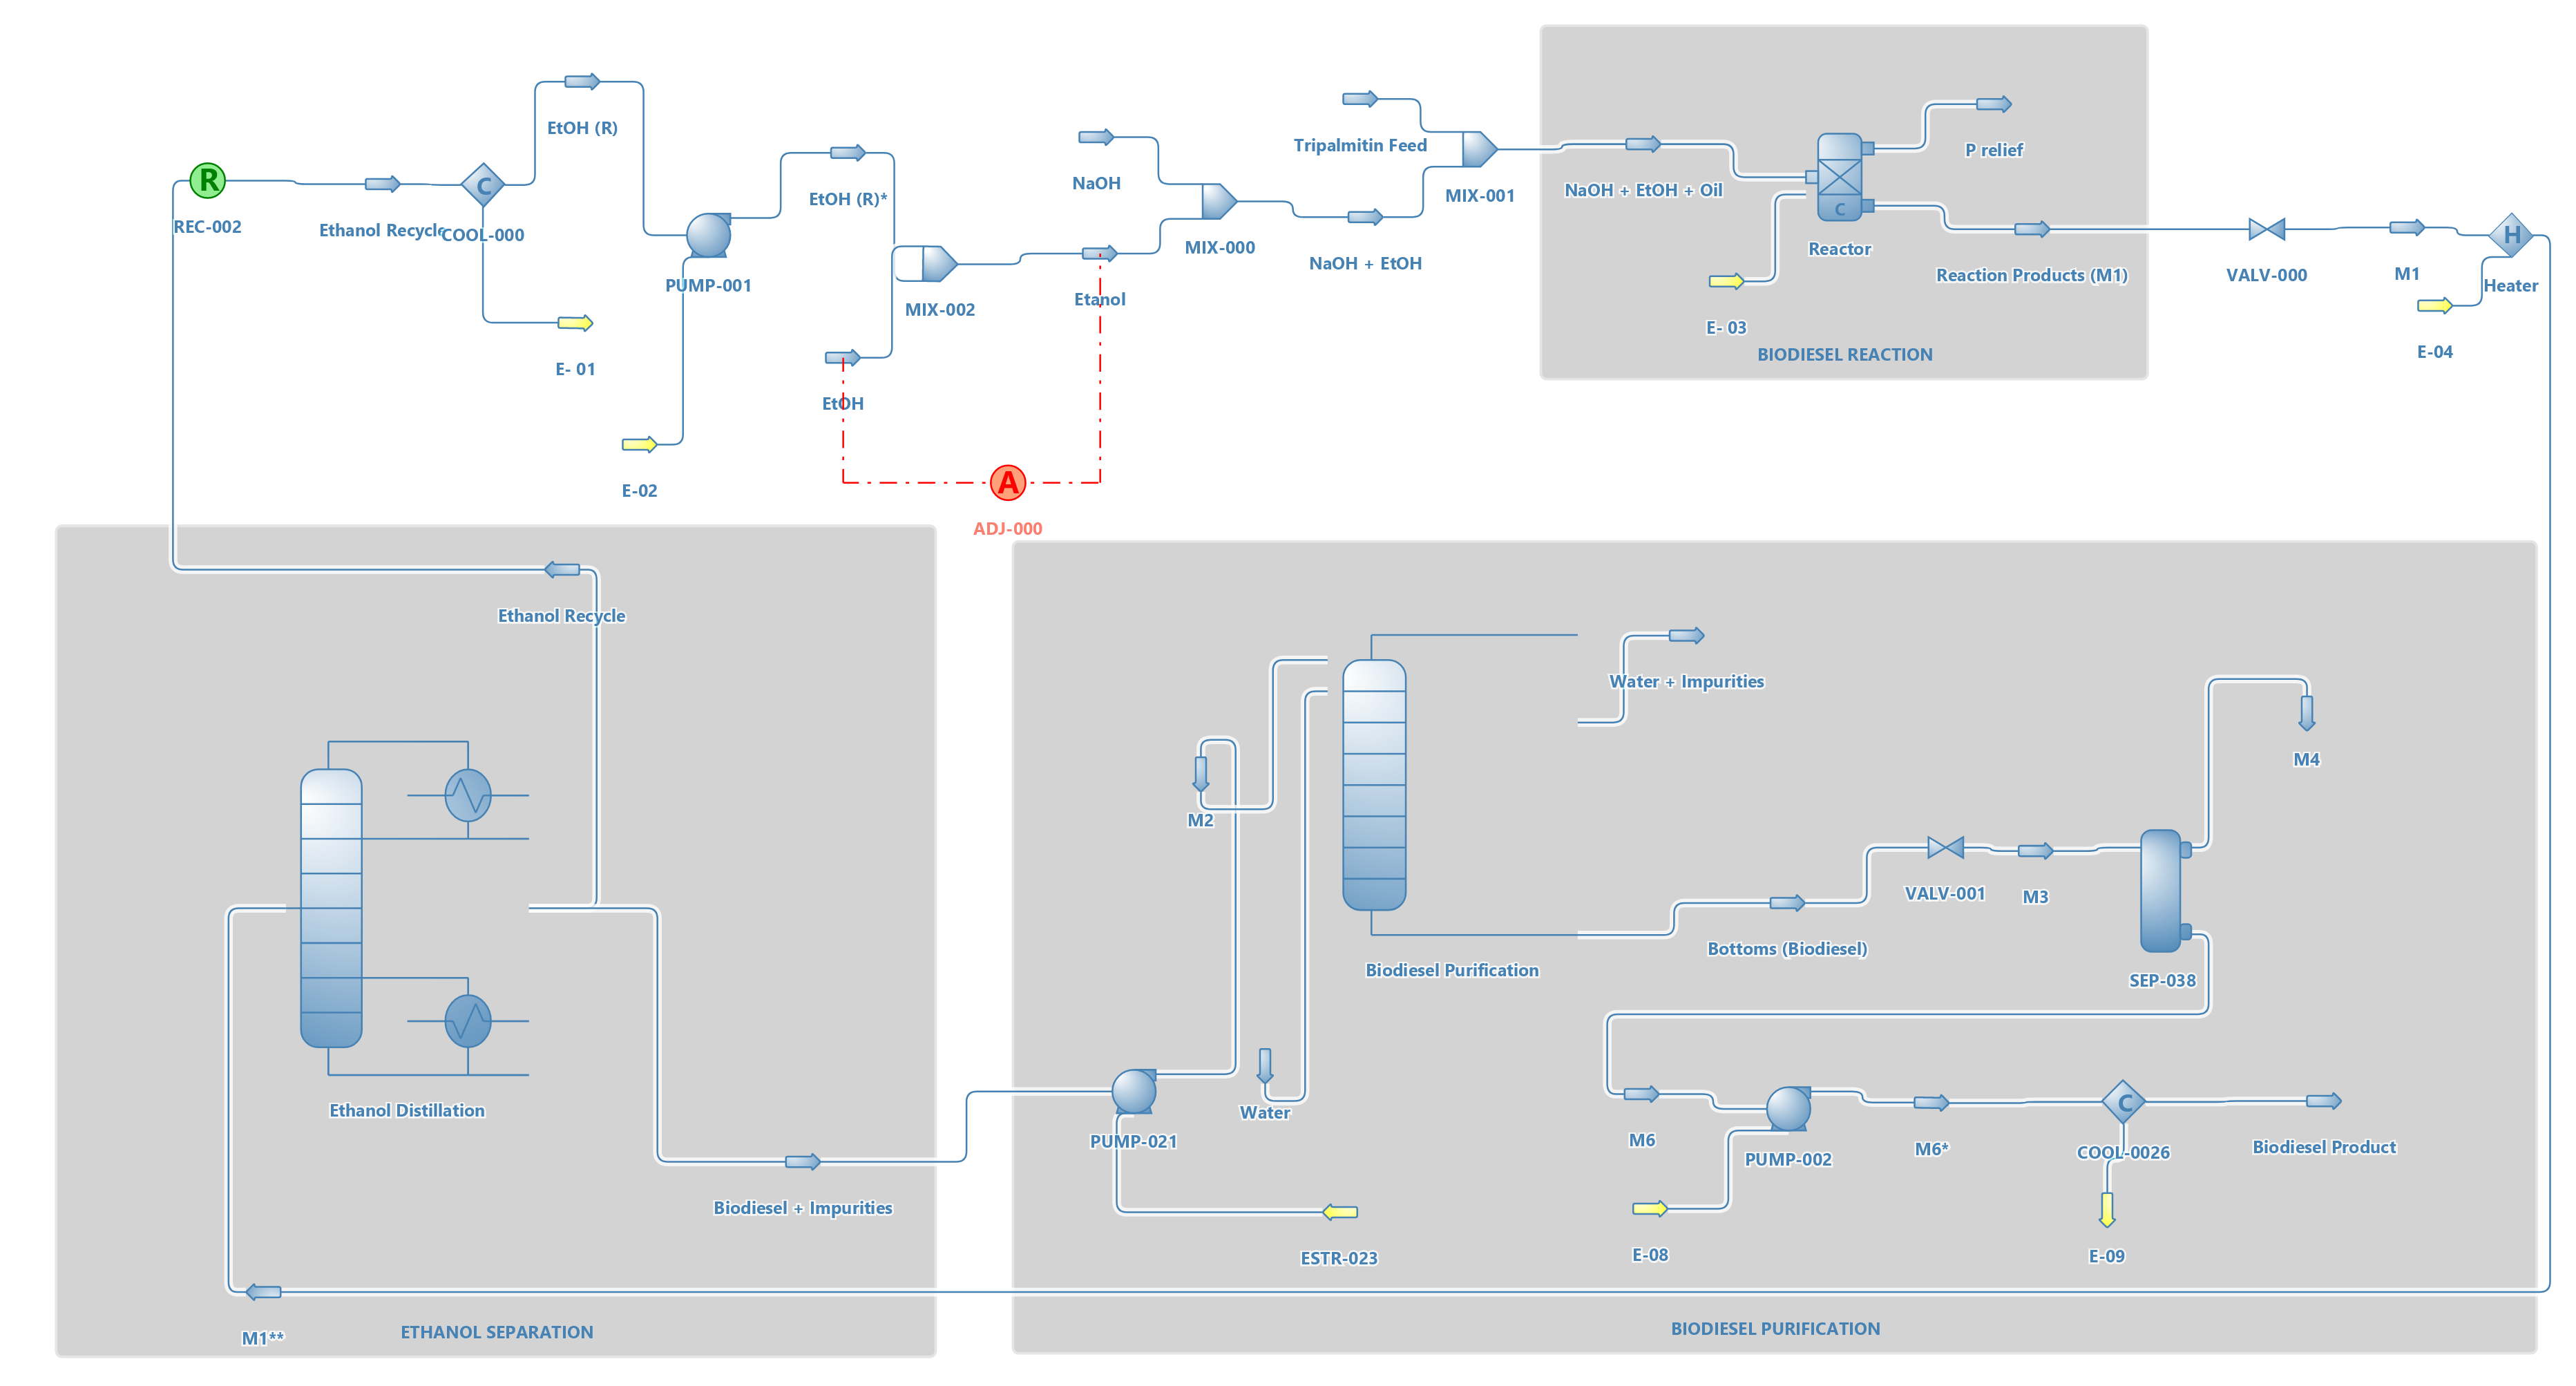
\includegraphics[width=1\linewidth]{Biodiesel-Prod.png}}

\newpage
\noindent \textbf{Results:}
\begin{table}[ht]
\centering
\resizebox{\textwidth}{!}{%
\begin{tabular}{|l|l|l|l|l|l|}
\hline
Object                                   & NaOH + EtOH & NaOH + EtOH + Oil & Reaction Products (M1) & M1**     &       \\ \hline
Temperature                              & 25.06392    & 51.07824          & 51.20892               & 44.67    & C     \\ \hline
Pressure                                 & 1           & 1                 & 1                      & 0.296077 & atm   \\ \hline
Mass Flow                                & 79.030073   & 303.2891          & 303.2891               & 303.2891 & g/s   \\ \hline
Molar Flow                               & 1.722756    & 2.000534          & 2.000539               & 2.000539 & mol/s \\ \hline
Mass Fraction (Mixture)  /  Ethanol\_BD  & 0.971569    & 0.253168          & 0.132914               & 0.132914 &       \\ \hline
Mass Fraction (Mixture)  /  EtP          & 0.000031    & 0.000008          & 0.742583               & 0.742583 &       \\ \hline
Mass Fraction (Mixture)  /  PPP          & 0           & 0.739423          & 0.036971               & 0.036971 &       \\ \hline
Mass Fraction (Mixture)  /  NaOH\_BD     & 0.028369    & 0.007392          & 0.007392               & 0.007392 &       \\ \hline
Mass Fraction (Mixture)  /  Glycerol\_BD & 0.000031    & 0.000008          & 0.080139               & 0.080139 &       \\ \hline
\end{tabular}%
}
\end{table}
\begin{table}[ht]
\centering
\resizebox{\textwidth}{!}{%
\begin{tabular}{|l|l|l|l|l|l|l|}
\hline
Object                                   & M1**       & Biodiesel + Impurities & Bottoms (Biodiesel) & Water + Impurities & Biodiesel Product &       \\ \hline
Temperature                              & 44.67      & 214.6771               & 60.00389            & 147.0185           & 25                & C     \\ \hline
Pressure                                 & 0.296077   & 0.296077               & 1                   & 1                  & 1                 & atm   \\ \hline
Mass Flow                                & 303.289073 & 263.5016               & 224.3065            & 305.2663           & 224.3065          & g/s   \\ \hline
Molar Flow                               & 2.000539   & 1.136907               & 0.781696            & 15.12477           & 0.781696          & mol/s \\ \hline
Mass Fraction (Mixture)  /  Ethanol\_BD  & 0.132914   & 0.001988               & 0.000519            & 0.001334           & 0.000519          &       \\ \hline
Mass Fraction (Mixture)  /  Water\_BD    & 0          & 0.09224                & 0                   & 0.871618           & 0                 &       \\ \hline
Mass Fraction (Mixture)  /  Glycerol\_BD & 0.080139   & 0.85471                & 0                   & 0.079613           & 0                 &       \\ \hline
Mass Fraction (Mixture)  /  EtP          & 0.742583   & 0.008509               & 0.982058            & 0.016165           & 0.982058          &       \\ \hline
Mass Fraction (Mixture)  /  NaOH\_BD     & 0.007392   & 0.042554               & 0                   & 0.007343           & 0                 &       \\ \hline
Mass Fraction (Mixture)  /  PPP          & 0.036971   & 0.042554               & 0.017423            & 0.023926           & 0.017423          &       \\ \hline
\end{tabular}%
}
\caption{Streamwise Results for Biodiesel Production}
\end{table}

\end{document}


